Use Venn diagrams to verify the following identities:
\begin{enumerate}[label=(\alph*)]
    \item $A \: \backslash \: (A \cap B) = A \: \backslash \: B$.
    \item $A \cup (B \cap C) = (A \cup B) \cap (A \cup C)$.
\end{enumerate}

\textbf{Solution:}
\begin{enumerate}[label=(\alph*)]
    \item Elements exclusively in $A$.\\
        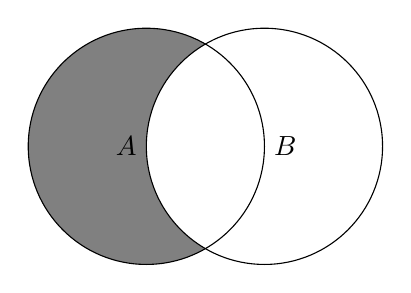
\begin{tikzpicture}
          % Define circles for A and B
          \def\circleA{(0,0) circle (1.5cm)}
          \def\circleB{(1.5,0) circle (1.5cm)}
        
          % Draw and fill A excluding the intersection with B
          \begin{scope}
            \clip \circleA;
            \fill[gray] \circleA;
            \clip \circleB;
            \fill[white] \circleA;
          \end{scope}
          
          % Outline the circles and label them
          \draw \circleA node [text=black, left] {$A$};
          \draw \circleB node [text=black, right] {$B$};
        \end{tikzpicture}

    \item Elements in $A$ or in the intersection of $B$ and $C$. \\
        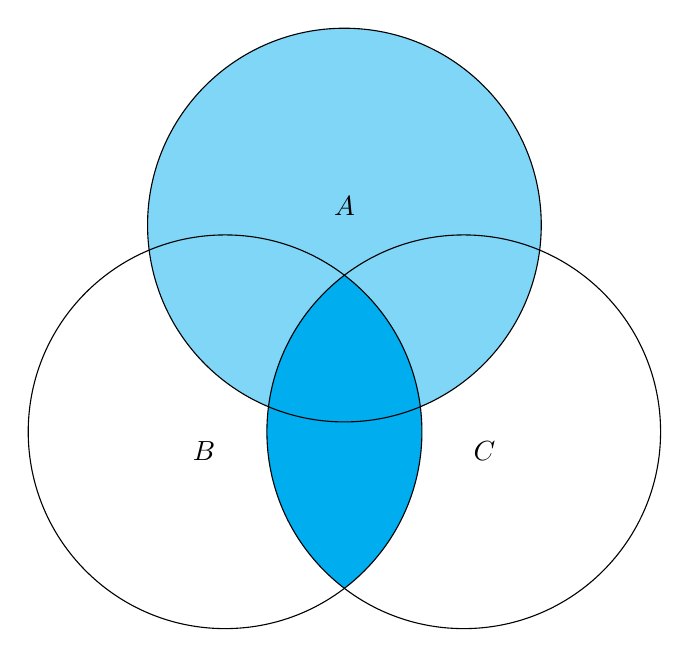
\begin{tikzpicture}
          % Define the circle paths for easier readability
          \def\firstcircle{(90:1.75cm) circle (2.5cm)}
          \def\secondcircle{(210:1.75cm) circle (2.5cm)}
          \def\thirdcircle{(330:1.75cm) circle (2.5cm)}
          
          % Shade intersection of B and C
          \begin{scope}
            \clip \secondcircle;
            \fill[cyan] \thirdcircle;
          \end{scope}
          
          % Shade A
          \fill[cyan, fill opacity=0.5] \firstcircle;
        
          % Draw the circles and add labels
          \draw \firstcircle node [text=black,above] {$A$};
          \draw \secondcircle node [text=black,below left] {$B$};
          \draw \thirdcircle node [text=black,below right] {$C$};
        \end{tikzpicture}
\end{enumerate}
\pagebreak